\chapter{CFG Abstract Semantics}
{\tt kr.ac.kaist.safe.analyzer}\\

Assumptions and limitations are as follows:
\begin{itemize}
    \item Semantics for helper functions is not written using denotational semantics
    (they are not compositional).
    \item For appropriate type conversion, a subscript is used. 
    In this case, all the implicit values can be considered as $\bot$.
    \item We maintain mutable inter-procedural edge set ($\ipnext$) throughout semantics.
\end{itemize}

\newpage
\section{Settings}
\[
\begin{array}{rlcl}
\acp, (n, \hat{cc}) \in & \aControlPoint & = & \SF{CFGNode} \times \abs{CallContext} \\
\hat{cc} \in & \abs{CallContext} &  & \comment{\inblue  Parameterized context-sensitivity.} \vspace{1mm}\\

\hat{S}, (\hat{H}, \hat{C}), \hat{E} \in & \aState & = &  \aHeap \times \aContext\\
\hat{H} \in & \aHeap & = & \aLoc \finto \aObj \vspace{1mm}\\
\hat{C} \in & \aContext & = &
%    \powerset{\aAddress} \times \powerset{\aAddress}
%    \comment{\inblue may old set, \ must old set} \\
\left\{ \begin{array}{rcl}
\emph{mayOld} & : & \powerset{\aAddress} \\
\emph{mustOld} & : & \powerset{\aAddress} \\
\end{array} \right\} \vspace{1mm}\\

\hat{l}_R,\hat{l}_O,\hat{l} \in & \aLoc &  = & \aAddress \times \abs{RecencyTag} \vspace{1mm}\\
\hat{a} \in & \aAddress & ::= & \avarloc{Global} ~\mid~ 
                                \avarloc{StringProto} ~\mid~ 
                                \avarloc{BooleanProto} ~\mid~ 
                                \avarloc{FunctionProto} \\
                          & & & ~\mid~m 
                                \avarloc{RefErr} ~\mid~ 
                                \avarloc{RangeErr} ~\mid~ 
                                \avarloc{TypeErr} ~\mid~ 
                                \avarloc{RefErrProto}  \\
                          & & & ~\mid~ 
                                 \avarloc{RangeErrProto} ~\mid~ 
                                 \avarloc{ArrayProto} ~\mid~ 
                                 \avarloc{TypeErrProto} \\
                          & & & ~\mid~ 
                                 \avarloc{ObjProto} ~\mid~ 
                                 \avarloc{PureLocal} ~\mid~ 
                                 \avarloc{GlobalCallsite} ~\mid~ 
                                 \avarloc{Collapsed} \\
                          & & & ~\mid~
                                 \hat{a}_1 ~\mid~ \cdots \\
    & \abs{RecencyTag} & ::= & \hat{Recent} \mid \hat{Old} \vspace{1mm}\\

\hat{o} \in & \aObj & = & \SF{Prop} \finto \abs{PropValue} \times \abs{Absent} \\
\hat{propv} \in & \abs{PropValue} & = & 
%    \abs{ObjectValue} \times \powerset{\fid} \\
\left\{ \begin{array}{rcl}
\emph{objval} & : & \abs{ObjectValue} \\
\emph{fidSet} & : & \powerset{\fid} \\
\end{array} \right\} \vspace{1mm}\\

\hat{objv} \in & \abs{ObjectValue} & = & 
%    \aValue \times \abs{Bool} \times \abs{Bool} \times \abs{Bool} \\
%    & & & {\inblue value,\ writable,\ enumerable,\ configurable} \\
\left\{ \begin{array}{rcl}
\emph{value} & : & \aValue \\
\emph{writable} & : & \abs{Bool} \\
\emph{enumerable} & : & \abs{Bool} \\
\emph{configurable} & : & \abs{Bool} \\
\end{array} \right\} \vspace{1mm}\\

\hat{v} \in & \aValue & = & 
%    \abs{PValue} \times \powerset{\aLoc} \\
\left\{ \begin{array}{rcl}
\emph{pvalue} & : & \abs{PValue} \\
\emph{locSet} & : & \powerset{\aLoc} \\
\emph{toAbsBool} & : & \SF{Unit} \rightarrow \abs{Bool}
\end{array} \right\} \vspace{1mm}\\

\hat{pv}\in & \abs{PValue} & = & 
%    \abs{Undef} \times \abs{Null} \times \abs{Bool} \times \abs{Number} \times \abs{String} \\
\left\{ \begin{array}{rcl}
\emph{undefVal} & : & \abs{Undef} \\
\emph{nullVal} & : & \abs{Null} \\
\emph{boolVal} & : & \abs{Bool} \\
\emph{numVal} & : & \abs{Number} \\
\emph{strVal} & : & \abs{String} \\
\end{array} \right\} \vspace{1mm}\\

\hat{exc}\in& \abs{Exception} & ::= & \hat{\exc{Error}} ~\mid~ 
                                      \hat{\exc{EvalError}} ~\mid~
                                      \hat{\exc{RangeError}} ~\mid~
                                      \hat{\exc{ReferenceError}} ~\mid~
                                      \hat{\exc{SyntaxError}} \\
                                & & & ~\mid~
                                      \hat{\exc{TypeError}} ~\mid~ 
                                      \hat{\exc{URIError}} \vspace{1mm}\\

\cfgnext, (\hat{cp}_1, \hat{cp}_2, \hat{C}, \hat{o}) \in & \abs{IPEdge} & = & 
    \aControlPoint \times \aControlPoint \times \abs{Context} \times \abs{Obj} \\
\ipnext\ \in & \powerset{\abs{IPEdge}} & & \\

\end{array}
\]

\newpage
\subsection{Shape of Data types}
\[
\abs{Undef} =
\begin{matrix}
  \begin{tikzpicture}
    \node (top) at (0,0) {$\aundef$};
    \node (down) at (0,-1.4) {$\bot_{\mbox{\scriptsize Undef}}$};
    \draw [black, thick, shorten <= -1pt, shorten >=-1pt] (top) -- (down);
  \end{tikzpicture}
\end{matrix}
\quad
\abs{Null} =
\begin{matrix}
  \begin{tikzpicture}
    \node (top) at (0,0) {$\anull$};
    \node (down) at (0,-1.4) {$\bot_{\mbox{\scriptsize Null}}$};
    \draw [black, thick, shorten <= -1pt, shorten >=-1pt] (top) -- (down);
  \end{tikzpicture}
\end{matrix}
\quad
\abs{Bool} =
\begin{matrix}
  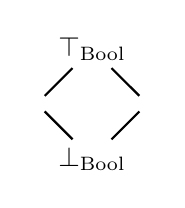
\begin{tikzpicture}
    \node (top) at (0,0) {$\top_{\mbox{\scriptsize Bool}}$};
    \node (midleft) at (-0.7,-0.7) {$\atrue$};
    \node (midright) at (0.7,-0.7) {$\afalse$};
    \node (down) at (0,-1.4) {$\bot_{\mbox{\scriptsize Bool}}$};
    \draw [black, thick, shorten <= -1pt, shorten >=-1pt] (top) -- (midleft);
    \draw [black, thick, shorten <= -1pt, shorten >=-1pt] (top) -- (midright);
    \draw [black, thick, shorten <= -1pt, shorten >=-1pt] (midleft) -- (down);
    \draw [black, thick, shorten <= -1pt, shorten >=-1pt] (midright) -- (down);
  \end{tikzpicture}
\end{matrix}
\quad
\abs{Absent} =
\begin{matrix}
  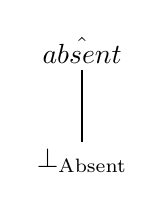
\begin{tikzpicture}
    \node (top) at (0,0) {$\hat{\SF{absent}}$};
    \node (down) at (0,-1.4) {$\bot_{\mbox{\scriptsize Absent}}$};
    \draw [black, thick, shorten <= -1pt, shorten >=-1pt] (top) -- (down);
  \end{tikzpicture}
\end{matrix}
\]
\[
\abs{Number} = 
\begin{matrix} 
  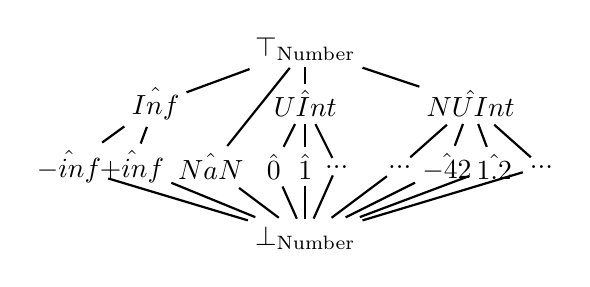
\begin{tikzpicture}
    % First, locate each of the nodes and name them
    \node (top) at (0,0) {$\top_{\mbox{\scriptsize Number}}$};
    \node (upperleft) at (-1.9,-0.7) {$\hat{\SF{Inf}}$};
    \node (uppercenter) at (0,-0.7) {$\hat{\SF{UInt}}$};
    \node (upperright) at (2.1,-0.7) {$\hat{\SF{NUInt}}$};
    \node (lower1) at (-3.0,-1.5) {$\hat{\SF{-inf}}$};
    \node (lower2) at (-2.2,-1.5) {$\hat{\SF{+inf}}$};
    \node (lower3) at (-1.2,-1.5) {$\hat{\SF{NaN}}$};
    \node (lower4) at (-0.4,-1.5) {$\hat{0}$};
    \node (lower5) at (0,-1.5) {$\hat{1}$};
    \node (lower6) at (0.4,-1.5) {...};
    \node (lower7) at (1.2,-1.5) {...};
    \node (lower8) at (1.8,-1.5) {$\hat{-42}$};
    \node (lower9) at (2.4,-1.5) {$\hat{1.2}$};
    \node (lower10) at (3,-1.5) {...};
    \node (down) at (0,-2.4) {$\bot_{\mbox{\scriptsize Number}}$};
    % Now draw the lines0
    \draw [black, thick, shorten <= -1pt, shorten >=-1pt] (top) -- (upperleft);
    \draw [black, thick, shorten <= -1pt, shorten >=-1pt] (top) -- (uppercenter);
    \draw [black, thick, shorten <= -1pt, shorten >=-1pt] (top) -- (upperright);
    \draw [black, thick, shorten <= -1pt, shorten >=-1pt] (top) -- (lower3);
    \draw [black, thick, shorten <= -1pt, shorten >=-1pt] (upperleft) -- (lower1);
    \draw [black, thick, shorten <= -1pt, shorten >=-1pt] (upperleft) -- (lower2);
    \draw [black, thick, shorten <= -1pt, shorten >=-1pt] (uppercenter) -- (lower4);
    \draw [black, thick, shorten <= -1pt, shorten >=-1pt] (uppercenter) -- (lower5);
    \draw [black, thick, shorten <= -1pt, shorten >=-1pt] (uppercenter) -- (lower6);
    \draw [black, thick, shorten <= -1pt, shorten >=-1pt] (upperright) -- (lower7);
    \draw [black, thick, shorten <= -1pt, shorten >=-1pt] (upperright) -- (lower8);
    \draw [black, thick, shorten <= -1pt, shorten >=-1pt] (upperright) -- (lower9);
    \draw [black, thick, shorten <= -1pt, shorten >=-1pt] (upperright) -- (lower10);
    \draw [black, thick, shorten <= -1pt, shorten >=-1pt] (lower1) -- (down);
    \draw [black, thick, shorten <= -1pt, shorten >=-1pt] (lower2) -- (down);
    \draw [black, thick, shorten <= -1pt, shorten >=-1pt] (lower3) -- (down);
    \draw [black, thick, shorten <= -1pt, shorten >=-1pt] (lower4) -- (down);
    \draw [black, thick, shorten <= -1pt, shorten >=-1pt] (lower5) -- (down);
    \draw [black, thick, shorten <= -1pt, shorten >=-1pt] (lower6) -- (down);
    \draw [black, thick, shorten <= -1pt, shorten >=-1pt] (lower7) -- (down);
    \draw [black, thick, shorten <= -1pt, shorten >=-1pt] (lower8) -- (down);
    \draw [black, thick, shorten <= -1pt, shorten >=-1pt] (lower9) -- (down);
    \draw [black, thick, shorten <= -1pt, shorten >=-1pt] (lower10) -- (down);
  \end{tikzpicture}
\end{matrix}
\]
\[
\abs{String} = 
	\begin{matrix} 
		\begin{tikzpicture}
	    % First, locate each of the nodes and name them
	    \node (top) at (0,0) {$\top_{\mbox{\scriptsize String}}$};
	    \node (upperleft) at (-1,-0.7) {$\hat{\SF{NumStr}}$};
	    \node (upperright) at (1,-0.7) {$\hat{\SF{OtherStr}}$};
	    \node (lower1) at (-2,-1.5) {$\hat{``\SF{NaN}"}$};
	    \node (lower2) at (-1.2,-1.5) {$\hat{``1.1"}$};
	    \node (lower3) at (-0.4,-1.5) {...};
	    \node (lower4) at (0.4,-1.5) {$\hat{``\mbox{foo}"}$};
	    \node (lower5) at (1.5,-1.5) {$\hat{``\mbox{bar}"}$};
	   	\node (lower6) at (2.2,-1.5) {...};
	    \node (down) at (0,-2.4) {$\bot_{\mbox{\scriptsize String}}$};
	    % Now draw the lines0
	  	\draw [black, thick, shorten <= -1pt, shorten >=-1pt] (top) -- (upperleft);
	  	\draw [black, thick, shorten <= -1pt, shorten >=-1pt] (top) -- (upperright);
	  	\draw [black, thick, shorten <= -1pt, shorten >=-1pt] (midleft) -- (lower1);
	  	\draw [black, thick, shorten <= -1pt, shorten >=-1pt] (midleft) -- (lower2);
	  	\draw [black, thick, shorten <= -1pt, shorten >=-1pt] (midleft) -- (lower3);
	  	\draw [black, thick, shorten <= -1pt, shorten >=-1pt] (midright) -- (lower4);
	  	\draw [black, thick, shorten <= -1pt, shorten >=-1pt] (midright) -- (lower5);
	  	\draw [black, thick, shorten <= -1pt, shorten >=-1pt] (midright) -- (lower6);
	  	\draw [black, thick, shorten <= -1pt, shorten >=-1pt] (lower1) -- (down);
	  	\draw [black, thick, shorten <= -1pt, shorten >=-1pt] (lower2) -- (down);
	  	\draw [black, thick, shorten <= -1pt, shorten >=-1pt] (lower3) -- (down);
	  	\draw [black, thick, shorten <= -1pt, shorten >=-1pt] (lower4) -- (down);
	  	\draw [black, thick, shorten <= -1pt, shorten >=-1pt] (lower5) -- (down);
	  	\draw [black, thick, shorten <= -1pt, shorten >=-1pt] (lower6) -- (down);
		\end{tikzpicture}
	\end{matrix}
\]

\newpage
\section{Domain Operators}
\subsection{Heap}
\subsection{Context}
\subsection{Obj}

\newpage
\section{Context-sensitivity}
\subsection{Context-insensitive}
\subsection{k-callsite-sensitive}

\newpage
\section{Helper Functions}

\subsection{Prunning Helper Functions}

\newpage
\section{Semantics}
\[
\begin{array}{lcl}
\aE & \in & \abs{IPEdge} \rightarrow \aState \rightarrow \aState \\
\aC & \in & \aControlPoint \rightarrow \aState \rightarrow \aState \times \aState\\
\aI & \in & \aControlPoint \rightarrow \SF{Instruction} 
    \rightarrow \aState \times \aState \rightarrow \aState \times \aState\\
\aV & \in & \SF{Expression} \rightarrow \aState 
    \rightarrow \aValue \times \powerset{\abs{Exception}} \\
\aB & \in & \SF{Expression} \rightarrow \aState \times \aState 
    \rightarrow \aState \times \aState\\
\end{array}
\]

\subsection{Interprocedural Edge}
\[
\renewcommand\arraystretch{1.5}
\begin{array}{l}
% call edge (bottom heap)
\aE \lbr ( \acp, (n \in \SF{Entry},\hat{cc}), \hat{C}, \hat{o} ) \rbr (\bot_{Heap},\hat{C}_1) 
    = \bot_{State}\\

% call edge
\aE \lbr ( \acp, (n \in \SF{Entry},\hat{cc}), \hat{C},\hat{o} ) \rbr (\hat{H}_1,\hat{C}_1) 
    = (\hat{H}_3,\hat{C}_1) \\
  \quad\wherec{
    \hat{H}_3 = \bigsqcup_{\hat{l}_{env}\in \hat{L}_{env}} \hat{H}_2[\hat{l}_{env} \mapsto \hat{o}_{env}]\\
    \land\ \hat{L}_{env} = \hat{o}_2(\varprop{env})\emph{.objval.value.locSet}\\
    \land\ \hat{H}_2 = \hat{H}_1[\avarloc{PureLocal}_R \mapsto \hat{o}_2] \\
    \land\ \hat{o}_2 = \hat{o} - \varprop{scope} \\
    \land\ \hat{o}_{env} = \ahf{NewDeclEnvRecord}(\hat{v}) \\
    \land\ \hat{v} = \hat{o}(\varprop{scope})\emph{.objval.value}
  }
\\\\

% normal return edge (bottom heap/context)
\aE \lbr ( (n \in \SF{Exit}, \hat{cc}), \acp, \hat{C},\hat{o} ) \rbr (\bot_{Heap}, \hat{C}_1)
    = \bot_{State}\\

\aE \lbr ( (n \in \SF{Exit}, \hat{cc}), \acp, \hat{C},\hat{o} ) \rbr (\hat{H}_1, \bot_{Context})
    = \bot_{State}\\

% normal return edge
\aE \lbr ( (n_1 \in \SF{Exit}, \hat{cc}_1), (n_2 \in \SF{AfterCall}, \hat{cc}_2), \hat{C}, \hat{o} ) \rbr (\hat{H}_1, \hat{C}_1)
   = \left\{
   \begin{array}{ll}
   \emph{\TT{new}\ State}(\hat{H}_3, \hat{C}_2) & \ifc{\hat{C}_2 \neq \bot_{Context}}\\
   \bot_{State} & \ifc{\hat{C}_2 = \bot_{Context}}\\
   \end{array}
   \right. \\
\quad\wherec{
    \hat{H}_3 = \ahf{VarStore}(\hat{H}_2, n_2\emph{.retVar}, \hat{v})\\
	\land\ \hat{H}_2 = \hat{H}_1[\avarloc{PureLocal} \mapsto \hat{o}_1]\\
	\land\ \hat{v} = \hat{H}_1(\avarloc{PureLocal})\\
	\land\ (\hat{C}_2, \hat{o}_1) = \ahf{FixOldify}(\hat{C},\ \hat{o},\ \hat{C}_1\emph{.mayOld},\ \hat{C}_1\emph{.mustOld})
}\\\\

\aE \lbr ( (n_1 \in \SF{Exit}, \hat{cc}_1), (n_2 \not\in \SF{AfterCall}, \hat{cc}_2), \hat{C}, \hat{o} ) \rbr\ \hat{S}
    \quad \comment{\inblue Impossible Case: IPFromExitToNoneError} \\

% exception return edge (bottom heap/context)
\aE \lbr ( (n \in \SF{ExitExc}, \hat{cc}), \acp, \hat{C},\hat{o} ) \rbr (\bot_{Heap}, \hat{C}_1)
    = \bot_{State}\\

\aE \lbr ( (n \in \SF{ExitExc}, \hat{cc}), \acp, \hat{C},\hat{o} ) \rbr (\hat{H}_1, \bot_{Context})
    = \bot_{State}\\

% exception return inter-procedural edge
\aE \lbr ( (n_1 \in \SF{ExitExc}, \hat{cc}_1), (n_2 \in \SF{AfterCatch}, \hat{cc}_2), \hat{C}, \hat{o} ) \rbr (\hat{H}_1, \hat{C}_1)
   = \left\{
   \begin{array}{ll}
   \emph{\TT{new}\ State}(\hat{H}_2, \hat{C}_2) & \ifc{\hat{C}_2 \neq \bot_{Context}}\\
   \bot_{State} & \ifc{\hat{C}_2 = \bot_{Context}}\\
   \end{array}
   \right. \\
\quad\wherec{
    \hat{H}_2 = \hat{H}_1 \left[ \avarloc{PureLocal} \mapsto 
        \hat{o}_1 \left[ \begin{array}{ll}
		    \varprop{exception} \mapsto \hat{v}_1, \\
			\varprop{exception\_all} \mapsto \hat{v}_1 \sqcup \hat{v}_2
		\end{array} \right] \right] \\
	\land\ \hat{v}_1 = \hat{H}_1(\avarloc{PureLocal})(\varprop{exception})\emph{.objval.value}\\
	\land\ \hat{v}_2 = \hat{o}_1(\varprop{exception\_all})\emph{.objval.value}\\
	\land\ (\hat{C}_2, \hat{o}_1) = \ahf{FixOldify}(\hat{C},\ \hat{o},\ \hat{C}_1\emph{.mayOld},\ \hat{C}_1\emph{.mustOld})
}\\\\

\aE \lbr ( (n_1 \in \SF{ExitExc}, \hat{cc}_1), (n_2 \not\in \SF{AfterCatch}, \hat{cc}_2), \hat{C}, \hat{o} ) \rbr\ \hat{S}
    \quad \comment{\inblue Impossible Case: IPFromExitToNoneError} \\

\end{array}
\]

\subsection{Block}
\[
\renewcommand\arraystretch{1.5}
\begin{array}{l}

\aC \lbr \hat{cp} \rbr\ \bot_{State} = (\bot_{State}, \bot_{State}) \\

% Entry Block
\aC \lbr (n \in \SF{Entry}, \hat{cc}) \rbr (\hat{H}_0, \hat{C}) = ((\hat{H}_m, \hat{C}), \bot_{State}) \\
\quad\wherec{
\forall n+1 \leq j \leq m.\ \hat{H}_j = \ahf{CreateMutableBinding}(\hat{H}_{j-1}, x_j, \abs{Value}(\aundef)) \\
\land\ \forall 1 \leq i \leq n.\ \hat{H}_i = \ahf{CreateMutableBinding}(\hat{H}_{i-1}, x_i,
    \bigsqcup_{\hat{l}_{arg} \in \hat{L}_{arg}}\ \ahf{Proto}(\hat{H}_{i-1}, \hat{l}_{arg}, \hat{``i-1"}) \\
\land\ x_{n+1} \cdots x_m = n\emph{.func.localVars} \
\land\ x_1 \cdots x_n = n\emph{.func.argVars} \\
\land\ \hat{L}_{arg} = \hat{H}_0(\avarloc{PureLocal})(n\emph{.func.argumentsName})\emph{.objval.value.locSet}
}\\\\

% Exit Block
\aC \lbr (n \in \SF{Exit}, \hat{cc}) \rbr\ \hat{S} = (\hat{S}, \bot_{State}) \\

% ExitExc Block
\aC \lbr (n \in \SF{ExitExc}, \hat{cc}) \rbr\ \hat{S} = (\hat{S}, \bot_{State}) \\

% Call Block
\aC \lbr (n \in \SF{Call}, \hat{cc}) \rbr\ \hat{S} 
= \aI_{(n, \hat{cc})} \lbr n\emph{.callInst} \rbr (\hat{S}, \bot_{State}) \\

% AfterCall Block
\aC \lbr (n \in \SF{AfterCall}, \hat{cc}) \rbr\ \hat{S} = (\hat{S}, \bot_{State}) \\

% AfterCatch Block
\aC \lbr (n \in \SF{AfterCatch}, \hat{cc}) \rbr\ \hat{S} = (\hat{S}, \bot_{State}) \\

% Normal Block
\aC \lbr (n \in \SF{Block}, \hat{cc}) \rbr\ \hat{S}_0 = (\hat{S}_n, \hat{E}_n) \\
\quad\wherec{
\forall 1 \leq k \leq n.\ 
(\hat{S}_k, \hat{E}_k) = \aI_{(n, \hat{cc})} \lbr i_k \rbr (\hat{S}_{k-1}, \hat{E}_{k-1}) \\
\land\ i_1 \cdots i_n = n\emph{.insts} \
\land\ \hat{E}_0 = \bot_{State}
}\\\\

\end{array}
\]

\subsection{Instruction}
\[
\renewcommand\arraystretch{1.5}
\begin{array}{l}

\aI_{\acp} \lbr i \rbr ((\bot_{Heap}, \hat{C}), \hat{S})  = (\bot_{State}, \hat{S}) \\\\

% CFGAlloc
\aI_{\acp} \lbr x~\verb+:=+~\TT{alloc}\verb+(+ \verb+)+_{\hat{a}} \rbr\ (\hat{S}, \hat{E}) = ((\hat{H}_3, \hat{C}_1), \hat{E}) \\
\quad\wherec{
\hat{H}_3 = \ahf{VarStore}(\hat{H}_2, x, \abs{Value}(\hat{l}_R)) \\
\land\ \hat{H}_2 = \ahf{AllocObject}(\hat{H}_1, \hat{L}_v, \hat{l}_R) \\
\land\ (\hat{H}_1, \hat{C}_1) = \ahf{Oldify}(\hat{S}, \hat{a}) \
\land\ \hat{l}_R = \emph{\TT{new} Loc}(\hat{a}, \hat{Recent}) \\
\land\ \hat{L}_v = \{\avarloc{ObjProto}\}
}\\\\

\aI_{\acp} \lbr x~\verb+:=+~\TT{alloc}\verb+(+ e \verb+)+_{\hat{a}} \rbr\ (\hat{S}, \hat{E}) = ((\hat{H}_3, \hat{C}_1), \hat{E}_1) \\
\quad\wherec{
\hat{H}_3 = \ahf{VarStore}(\hat{H}_2, x, \abs{Value}(\hat{l}_R)) \\
\land\ \hat{H}_2 = \ahf{AllocObject}(\hat{H}_1, \hat{L}_v, \hat{l}_R) \\
\land\ (\hat{H}_1, \hat{C}_1) = \ahf{Oldify}(\hat{S}, \hat{a}) \
\land\ \hat{l}_R = \emph{\TT{new} Loc}(\hat{a}, \hat{Recent}) \\
\land\ \hat{L}_v = 
    \left \{ \begin{array}{ll} 
	\hat{v}\emph{.locSet} & \ifc{\hat{v}\emph{.pvalue} \not\sqsubseteq \bot_{PValue}}\\
	\hat{v}\emph{.locSet}\ \cup\ \{\avarloc{ObjProto}\} & \owc \\
	\end{array} \right.\\
\land\ \hat{E}_1 = \hat{E} + \ahf{RaiseException}(\hat{S}, \hat{es}) \\
\land\ (\hat{v}, \hat{es}) = \aV \lbr e \rbr\ (\hat{H}_1, \hat{C}_1)
}\\\\

\end{array}
\]

\[
\renewcommand\arraystretch{1.5}
\begin{array}{l}


% CFGAllocArray
\aI_{\acp} \lbr x~\verb+:=+~\TT{allocArray}\verb+(+n\verb+)+_{\hat{a}} \rbr\ (\hat{S}, \hat{E}) = ((\hat{H}_3, \hat{C}_1), \hat{E}) \\
\quad\wherec{
\hat{H}_3 = \ahf{VarStore}(\hat{H}_2, x, \abs{Value}(\hat{l}_R)) \\
\land\ \hat{H}_2 = \hat{H}_1 [\hat{l}_R \mapsto \ahf{NewArrayObject}(\hat{n})] \\
\land\ (\hat{H}_1, \hat{C}_1) = \ahf{Oldify}(\hat{S}, \hat{a}) \
\land\ \hat{l}_R = \emph{\TT{new} Loc}(\hat{a}, \hat{Recent}) \\
\land\ \hat{n} = \hat{v}\emph{.pvalue.numVal} \
\land\ (\hat{v}, -) = \aV \lbr e \rbr\ (\hat{H}_1, \hat{C}_1)
}\\\\

% CFGAllocArg
\aI_{\acp} \lbr x~\verb+:=+~\TT{allocArg}\verb+(+n\verb+)+_{\hat{a}} \rbr\ (\hat{S}, \hat{E}) = ((\hat{H}_3, \hat{C}_1), \hat{E}) \\
\quad\wherec{
\hat{H}_3 = \ahf{VarStore}(\hat{H}_2, x, \abs{Value}(\hat{l}_R)) \\
\land\ \hat{H}_2 = \hat{H}_1 [\hat{l}_R \mapsto \ahf{NewArgObject}(\hat{n})] \\
\land\ (\hat{H}_1, \hat{C}_1) = \ahf{Oldify}(\hat{S}, \hat{a}) \
\land\ \hat{l}_R = \emph{\TT{new} Loc}(\hat{a}, \hat{Recent}) \\
\land\ \hat{n} = \hat{v}\emph{.pvalue.numVal} \
\land\ (\hat{v}, -) = \aV \lbr e \rbr\ (\hat{H}_1, \hat{C}_1)
}\\\\

% CFGExprStmt
\aI_{\acp} \lbr x ~\verb+:=+~ e \rbr\ ((\hat{H}, \hat{C}), \hat{E}) = ((\hat{H}_1, \hat{C}_1), \hat{E}_1) \\
\quad\wherec{
(\hat{H}_1, \hat{C}_1) = \left \{ \begin{array}{ll}
(\ahf{VarStore}(\hat{H}, x, \hat{v}),\ \hat{C}) & \ifc{\hat{v} \not\sqsubseteq \bot_{Value}}\\
(\bot_{Heap}, \bot_{Context}) & \owc \\
\end{array} \right.\\
\land\ \hat{E}_1 = \hat{E} \sqcup \ahf{RaiseException}((\hat{H}, \hat{C}),\ \hat{es}) \\
\land\ (\hat{v}, \hat{es}) = \aV \lbr e \rbr (\hat{H}, \hat{C})
}\\\\

% CFGDelete
\aI_{\acp} \lbr x_1 ~\verb+:=+~ \TT{delete}\verb+(+x_2\verb+)+ \rbr\ ((\hat{H}, \hat{C}), \hat{E}) = ((\hat{H}_2, \hat{C}), \hat{E}) \\
\quad\wherec{
\hat{H}_2 = \ahf{VarStore}(\hat{H}_1,\ x_1,\ \abs{Value}(\hat{b})) \\
\land\ (\hat{H}_1, \hat{b}) = \left \{ \begin{array}{ll}
(\hat{H}, \atrue) & \ifc{\hat{L}_{base} = \varnothing} \\
\bigsqcup_{\hat{l} \in \hat{L}_{base}} \ahf{Delete}(\hat{H},\ \hat{l},\ \hat{x_2}) & \owc \\
\end{array} \right. \\
\land\ \hat{L}_{base} = \ahf{LookupBase}(\hat{H},\ x_2)
}\\\\

\aI_{\acp} \lbr x ~\verb+:=+~ \TT{delete}\verb+(+e\verb+)+ \rbr\ ((\hat{H}, \hat{C}), \hat{E}) = ((\hat{H}_1, \hat{C}_1), \hat{E}_1) \\
\quad\wherec{
(\hat{H}_1, \hat{C}_1) = \left \{ \begin{array}{ll}
(\ahf{VarStore}(\hat{H},\ x,\ \abs{Value}(\atrue),\ \hat{C}) & \ifc{ \hat{v} \not\sqsubseteq \bot_{Value}} \\
(\bot_{Heap},\ \bot_{Context}) & \owc \\
\end{array} \right.\\
\land\ \hat{E}_1 = \hat{E} \sqcup \ahf{RaiseException}((\hat{H}, \hat{C}), \hat{es}) \\
\land\ (\hat{v}, \hat{es}) = \aV \lbr e \rbr (\hat{H}, \hat{C})
}\\\\

% CFGDeleteProp
\aI_{\acp} \lbr x ~\verb+:=+~ \TT{delete}\verb+(+e_1,e_2\verb+)+ \rbr\ ((\hat{H}, \hat{C}), \hat{E}) = ((\hat{H}_2, \hat{C}_2), \hat{E}_1) \\
\quad\wherec{
(\hat{H}_2, \hat{C}_2) = \left \{ \begin{array}{ll}
(\ahf{VarStore}(\hat{H}_1,\ x,\ \abs{Value}(\hat{b})),\ \hat{C}) & \ifc{\hat{H}_1 \not\sqsubseteq \bot_{Heap}} \\
(\bot_{Heap}, \bot_{Context}) & \owc \\
\end{array} \right.\\
\land\ (\hat{H}_1, \hat{b}) = \left \{ \begin{array}{ll}
\bigsqcup_{\hat{l} \in \hat{v}_1\emph{.locSet}} \bigsqcup_{\hat{s} \in S_{idx}} \ahf{Delete}(\hat{H},\ \hat{l},\ \hat{s}) 
    & \ifc{\hat{v}_1\emph{.locSet} \neq \varnothing \land\ S_{idx} \neq \varnothing} \\
(\bot_{Heap}, \bot_{Bool}) & \owc \\
\end{array} \right. \\
\land\ \hat{E}_1 = \hat{E} \sqcup \ahf{RaiseException}((\hat{H}, \hat{C}), \hat{es}) \\
\land\ S_{idx} = \left \{ \begin{array}{ll}
\ahf{toStringSet}(\ahf{toPrimitiveBetter}(\hat{H}, \hat{v}_2)) & \ifc{\hat{v}_2 \not\sqsubseteq \bot_{Value}} \\
\varnothing & \owc \\
\end{array} \right.\\
\land\ (\hat{v}_1, -) = \aV \lbr e_1 \rbr (\hat{H}, \hat{C}) \
\land\ (\hat{v}_2, \hat{es}) = \aV \lbr e_2 \rbr (\hat{H}, \hat{C})
}\\\\

\end{array}
\]

\[
\renewcommand\arraystretch{1.5}
\begin{array}{l}

% CFGStore
\aI_{\acp} \lbr e\verb+[+s\verb+]+ ~\verb+:=+~ e \rbr\ (\hat{S}, \hat{E}) \\
\aI_{\acp} \lbr e\verb+[+e\verb+]+ ~\verb+:=+~ e \rbr\ (\hat{S}, \hat{E}) \\


\end{array}
\]

\[
\renewcommand\arraystretch{1.5}
\begin{array}{l}

% CFGFunExpr
\aI_{\acp} \lbr x ~\verb+:=+~ \TT{function} ~\verb+(+f\verb+)+_{\hat{a}_1, \hat{a}_2} \rbr\ (\hat{S}, \hat{E}) 
= ((\hat{H}_5, \hat{C}_2), \hat{E}) \\
\quad\wherec{
\hat{H}_5 = \ahf{VarStore}(\hat{H}_4,\ x,\ \abs{Value}(\hat{l}_{R1})) \\
\land\ \hat{H}_4 = \hat{H}_3 \left[\hat{l}_{R2} \mapsto \hat{o}_{new}
\left[``constructor" \mapsto \langle \abs{Value}(\hat{l}_{R1}),\ \atrue,\ \afalse,\ \atrue \rangle \right]
\right] \\
\land\ \hat{H}_3 = \hat{H}_2 
\left[\hat{l}_{R1} \mapsto \ahf{NewFunctionObject}(fid,\ \hat{v}_{env},\ \hat{l}_{R2},\ \hat{n}) \right] \\
\land\ (\hat{H}_2, \hat{C}_2) = \ahf{Oldify}(\hat{S}_1, \hat{a}_2) \
\land\ \hat{S}_1 = \ahf{Oldify}(\hat{S}, \hat{a}_1) \\
\land\ \hat{l}_{R1} = \emph{\TT{new} Loc}(\hat{a}_1, \hat{Recent}) \
\land\ \hat{l}_{R2} = \emph{\TT{new} Loc}(\hat{a}_2, \hat{Recent}) \\
\land\ \hat{o}_{new} = \ahf{NewObject}(\avarloc{ObjectProto})\\
\land\ \hat{v}_{env} = \hat{H}_2(\avarloc{PureLocal})(\varprop{env})\emph{.objval.value} \\
\land\ \hat{n} = f\emph{.argVars.length} \\
}\\\\

\aI_{\acp} \lbr x_1 ~\verb+:=+~ \TT{function} ~x_2 \verb+(+f\verb+)+_{\hat{a}_1,\ \hat{a}_2,\ \hat{a}_3} \rbr\ (\hat{S}, \hat{E}) = ((\hat{H}_7, \hat{C}_3), \hat{E}) \\
\quad\wherec{
\land\ \hat{H}_7 = \ahf{VarStore}(\hat{H}_6, x_1, \abs{Value}(\hat{l}_{R1})) \\
\land\ \hat{H}_6 = \hat{H}_5 \left[ \hat{l}_{R3} \mapsto \hat{o}_{env}
\left[ x_2 \mapsto \langle \abs{Value}(\hat{l}_{R1}),\ \afalse,\ \bot_{Bool},\ \afalse \rangle \right]
\right] \\
\land\ \hat{H}_5 = \hat{H}_4 \left[ \hat{l}_{R2} \mapsto \hat{o}_{new} 
\left[ ``constructor" \mapsto \langle \abs{Value}(\hat{l}_{R1}),\ \atrue,\ \afalse,\ \atrue \rangle \right]
\right] \\
\land\ \hat{H}_4 = \hat{H}_3 
\left[ \hat{l}_{R3} \mapsto \ahf{NewFunctionObject}(fid,\ \abs{Value}(\hat{l}_{R3},\ \hat{l}_{R2},\ \hat{n})) \right] \\
\land\ (\hat{H}_3, \hat{C}_3) = \ahf{Oldify}(\hat{S}_2, \hat{a}_3) \
\land\ \hat{S}_2 = \ahf{Oldify}(\hat{S}_1, \hat{a}_2) \
\land\ \hat{S}_1 = \ahf{Oldify}(\hat{S}, \hat{a}_1) \\
\land\ \hat{l}_{R1} = \emph{\TT{new} Loc}(\hat{a}_1, \hat{Recent}) \
\land\ \hat{l}_{R2} = \emph{\TT{new} Loc}(\hat{a}_2, \hat{Recent}) \
\land\ \hat{l}_{R3} = \emph{\TT{new} Loc}(\hat{a}_3, \hat{Recent}) \\
\land\ \hat{o}_{env} = \ahf{NewDeclEnvRecord}(\hat{v}_{env}) \
\land\ \hat{o}_{new} = \ahf{NewObject}(\avarloc{ObjectProto}) \\
\land\ \hat{v}_{env} = \hat{H}_3(\avarloc{PureLocal})(\varprop{env})\emph{.objval.value} \\
\land\ \hat{n} = f\emph{.argVars.length} \\
}\\\\

% CFGReturn
\aI_{\acp} \lbr \TT{return} \rbr\ ((\hat{H}, \hat{C}), \hat{E}) = ((\hat{H}_1, \hat{C}), \hat{E}) \\
\quad\wherec{
\hat{H}_1 = \hat{H} \left[ \avarloc{PureLocal} \mapsto
\hat{o} \left[ \varprop{return} \mapsto \abs{PropValue}(\aundef) \right] \right]
}\\\\

\aI_{\acp} \lbr \TT{return}\verb+(+e\verb+)+ \rbr\ ((\hat{H}, \hat{C}), \hat{E}) = ((\hat{H}_1, \hat{C}_1), \hat{E}_1) \\
\quad\wherec{
(\hat{H}_1, \hat{C}_1) = \left \{ \begin{array}{ll}
(\hat{H} \left[ \avarloc{PureLocal} \mapsto
\hat{o} \left[ \varprop{return} \mapsto \abs{PropValue}(\hat{v}) \right] \right],\ \hat{C})
& \ifc {\hat{v} \not\sqsubseteq \bot_{Value}} \\
(\bot_{Heap}, \bot_{Context}) & \owc \\
\end{array}\right. \\
\land\ \hat{E}_1 = \hat{E} \sqcup \ahf{RaiseException}((\hat{H}, \hat{C}), \hat{es}) \\
\land\ (\hat{v}, \hat{es}) = \aV \lbr e \rbr (\hat{H}, \hat{C})
}\\\\

\end{array}
\]

\[
\renewcommand\arraystretch{1.5}
\begin{array}{l}

% CFGCall
\aI_{\acp} \lbr \TT{call}\verb+(+e_1,e_2,e_3\verb+)+ \rbr\ (\hat{S}, \hat{E}) \\

% CFGConstruct
\aI_{\acp} \lbr \TT{construct}\verb+(+e_1,e_2,e_3\verb+)+ \rbr\ (\hat{S}, \hat{E}) \\

\end{array}
\]

\[
\renewcommand\arraystretch{1.5}
\begin{array}{l}

% CFGAssert
\aI_{\acp} \lbr \TT{assert}\verb+(+e\inop e\verb+)+ \rbr\ (\hat{S}, \hat{E}) 
= \aB \lbr \verb+(+e\inop e\verb+)+ \rbr\ (\hat{S}, \hat{E}) \\\\

% CFGCatch
\aI_{\acp} \lbr \TT{catch}\verb+(+x\verb+)+ \rbr\ ((\hat{H}, \hat{C}), \hat{E}) = ((\hat{H}_2, \hat{C}), \bot_{State}) \\
\quad\wherec{
\hat{H}_2 = \left[ \avarloc{PureLocal} \mapsto \hat{H}_1(\avarloc{PureLocal})
\left[ \varprop{exception} \mapsto \hat{o}_{es} \right] \right]\\
\land\ \hat{H}_1 = \ahf{CreateMutableBinding}(\hat{H}, x, \hat{o}_e\emph{.objval.value}) \\
\land\ \hat{o}_{es} = \hat{H}(\avarloc{PureLocal})(\varprop{exception\_all}) \\
\land\ \hat{o}_e = \hat{H}(\avarloc{PureLocal})(\varprop{exception}) \\
}\\\\

% CFGThrow
\aI_{\acp} \lbr \TT{throw}\verb+(+e\verb+)+ \rbr\ ((\hat{H}, \hat{C}), \hat{E}) = (\bot_{State}, \hat{E}_1) \\
\quad\wherec{
\hat{E}_1 = \hat{E} \sqcup (\hat{H}_1, \hat{C}) \sqcup \ahf{RaiseException}((\hat{H}, \hat{C}), \hat{es}) \\
\land\ \hat{H}_1 = \hat{H} \left[ \avarloc{PureLocal} \mapsto \left[ \begin{array}{ll}
\varprop{exception} \mapsto \abs{PropValue}(\hat{v}), \\
\varprop{exception\_all} \mapsto \abs{PropValue}(\hat{v} \sqcup \hat{o}_{es}\emph{.objval.value}), \\
\varprop{return} \mapsto \abs{PropValue}(\aundef) \\
\end{array} \right] \right]\\
\land\ \hat{o}_{es} = \hat{H}(\avarloc{PureLocal})(\varprop{exception\_all}) \\
\land\ (\hat{v}, \hat{es}) = \aV \lbr e \rbr (\hat{H}, \hat{C})
}\\\\

% CFGNoOp
\aI_{\acp} \lbr \TT{noop} \rbr\ (\hat{S}, \hat{E}) = (\hat{S}, \hat{E}) \\\\

% CFGInternalCall <>toObject
\aI_{\acp} \lbr x ~\verb+:=+~\ahf{\ensuremath{\diamond}toObject}\verb+(+e\verb+)+ \rbr\ (\hat{S}, \hat{E}) \\

% CFGInternalCall <>isObject
\aI_{\acp} \lbr x ~\verb+:=+~\ahf{\ensuremath{\diamond}isObject}\verb+(+e\verb+)+ \rbr\ (\hat{S}, \hat{E}) \\

% CFGInternalCall <>toNumber
\aI_{\acp} \lbr x ~\verb+:=+~\ahf{\ensuremath{\diamond}toNumber}\verb+(+e\verb+)+ \rbr\ (\hat{S}, \hat{E}) \\

% CFGInternalCall <>toBoolean
\aI_{\acp} \lbr x ~\verb+:=+~\ahf{\ensuremath{\diamond}toBoolean}\verb+(+e\verb+)+ \rbr\ (\hat{S}, \hat{E}) \\

% CFGInternalCall <>getBase
\aI_{\acp} \lbr x ~\verb+:=+~\ahf{\ensuremath{\diamond}getBase}\verb+(+x\verb+)+ \rbr\ (\hat{S}, \hat{E}) \\

% CFGInternalCall <>iteratorInit
\aI_{\acp} \lbr x ~\verb+:=+~\ahf{\ensuremath{\diamond}iteratorInit}\verb+(+e_1\verb+)+_{\hat{a}} \rbr\ (\hat{S}, \hat{E}) \\

% CFGInternalCall <>iteratorHasNext
\aI_{\acp} \lbr x ~\verb+:=+~\ahf{\ensuremath{\diamond}iteratorHasNext}\verb+(+e_1,\ e_2\verb+)+ \rbr\ (\hat{S}, \hat{E}) \\

% CFGInternalCall <>iteratorNext
\aI_{\acp} \lbr x ~\verb+:=+~\ahf{\ensuremath{\diamond}iteratorNext}\verb+(+e_1,\ e_2\verb+)+ \rbr\ (\hat{S}, \hat{E}) \\

\end{array}
\]

\subsection{Expression}
\[
\renewcommand\arraystretch{1.5}
\begin{array}{l}

\aV \lbr x \rbr\ \hat{S} \\
\aV \lbr e \inop e \rbr\ \hat{S} \\
\aV \lbr \preop e \rbr\ \hat{S} \\
\aV \lbr e\verb+[+e\verb+]+ \rbr\ \hat{S} \\
\aV \lbr \TT{this} \rbr\ \hat{S} \\
\aV \lbr n \rbr\ \hat{S} \\
\aV \lbr ``s" \rbr\ \hat{S} \\
\aV \lbr \TT{true} \rbr\ \hat{S} \\
\aV \lbr \TT{false} \rbr\ \hat{S} \\
\aV \lbr \TT{null} \rbr\ \hat{S} \\

\end{array}
\]

\subsection{Assertion}
\[
\renewcommand\arraystretch{1.5}
\begin{array}{l}

\aB \lbr e \rbr (\hat{S}_1, \hat{E}_1) 
    = (\emph{\TT{new}\ State}(\hat{H}_2, \hat{S}_1\emph{.context}), \hat{E}_3) \\
\quad\wherec{
    \hat{H}_2 = \left \{
	\begin{array}{ll}
        \hat{S}_1\emph{.heap} & \ifc{\hat{true} \sqsubseteq \hat{v}\emph{.toAbsBool}} \\
	    \bot_{Heap} & \owc
    \end{array}  \right.\\
    \land\ \hat{E}_3 = \hat{E}_1 \sqcup \hat{E}_2 \\
    \land\ \hat{E}_2 = \chf{RaiseException}(\hat{S}_1, \hat{es}) \\
	\land\ (\hat{v}, \hat{es}) = \aV \lbr e \rbr\ \hat{S}_1
}\\\\

\end{array}
\]
